\subsubsection{Adding Backgorund}
    Background images are those that do not have an object that needs to be classified to reduce False Positives (FP).
    Small chunks of background images are added to the training, validation, and testing datasets in addition to labeled images.
    As the background image fraction approaches 1.0, the training process will suffer.
    Background images should have a maximum proportion of 10 percent, as recommended by the author of YOLO5.
    In this project, background should be scenery images\cite{addingbackgroundimages}. 
    \begin{figure}[H]
    \centering
    \begin{subfigure}{0.241\textwidth}
        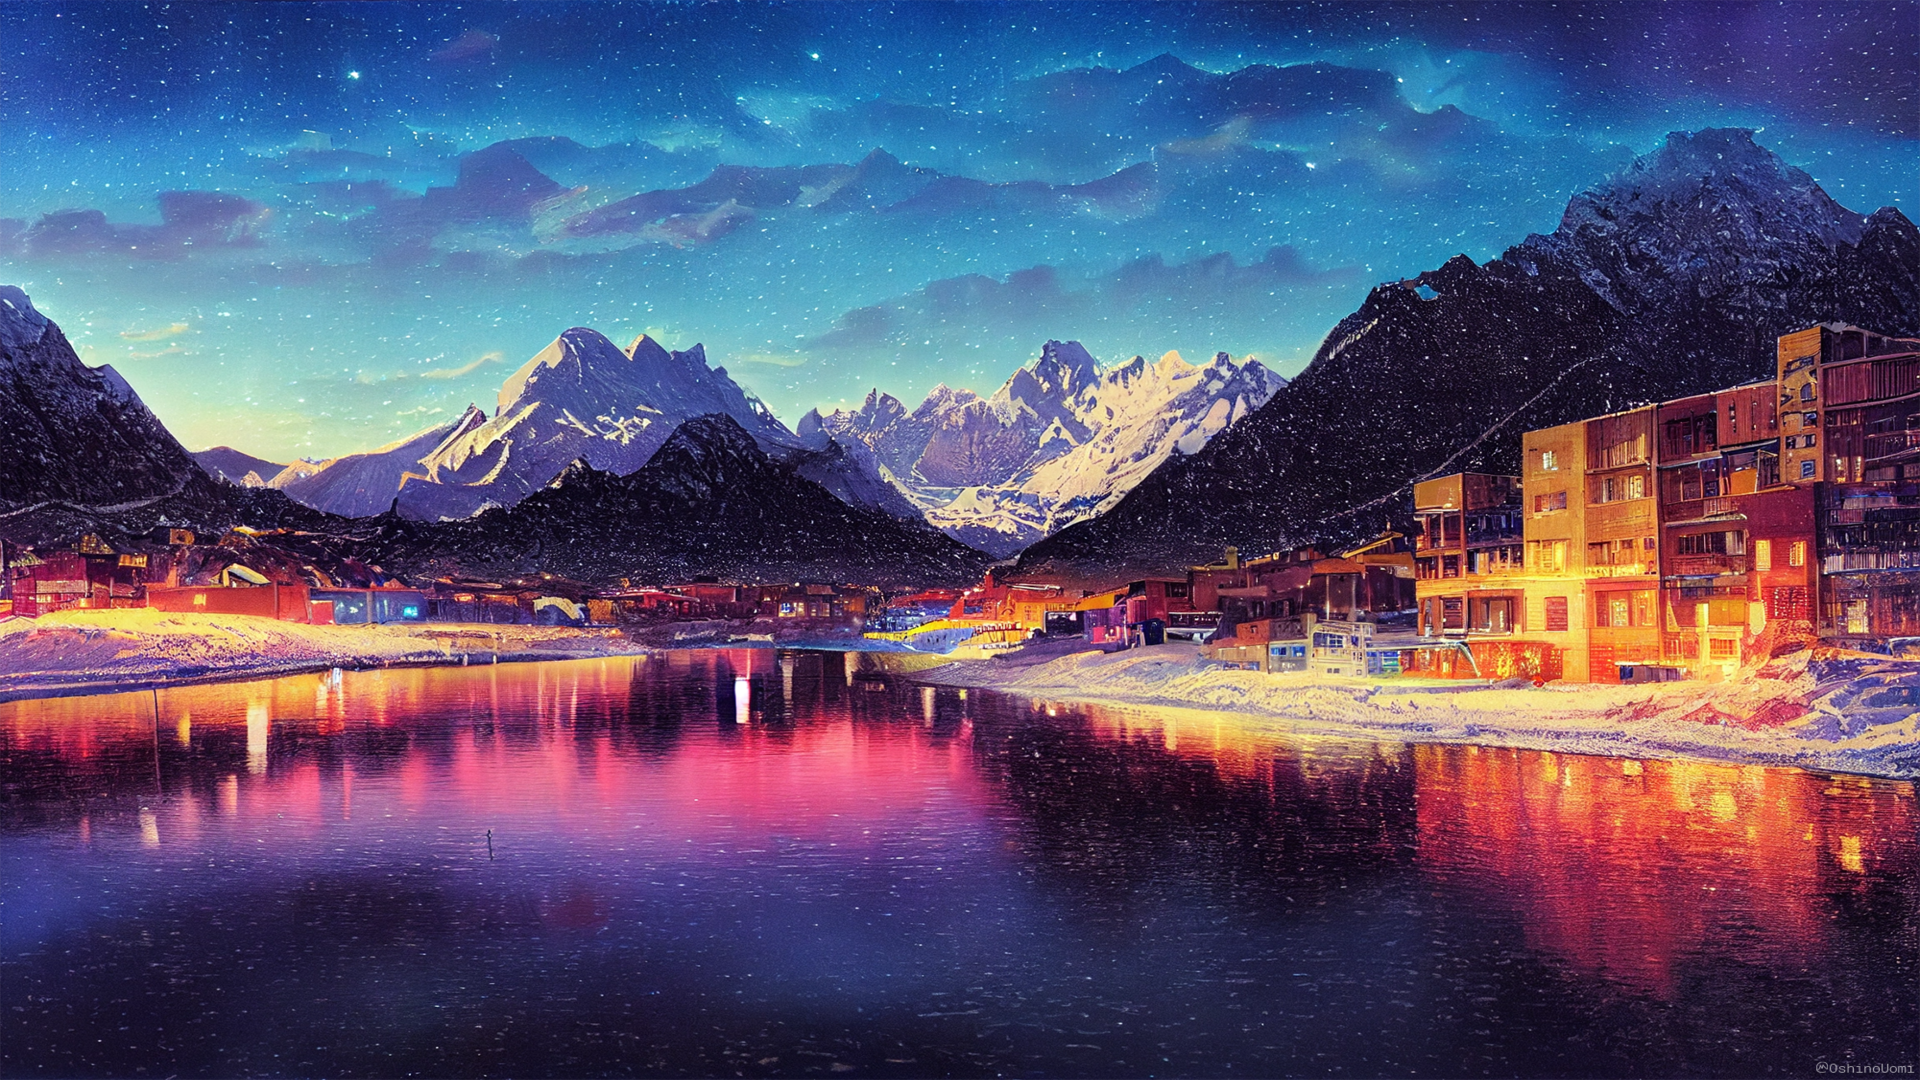
\includegraphics[width=1\textwidth]{images/background/Pixiv-101510980_p0.png}
    \end{subfigure}
    \hfill
    \begin{subfigure}{0.241\textwidth}
        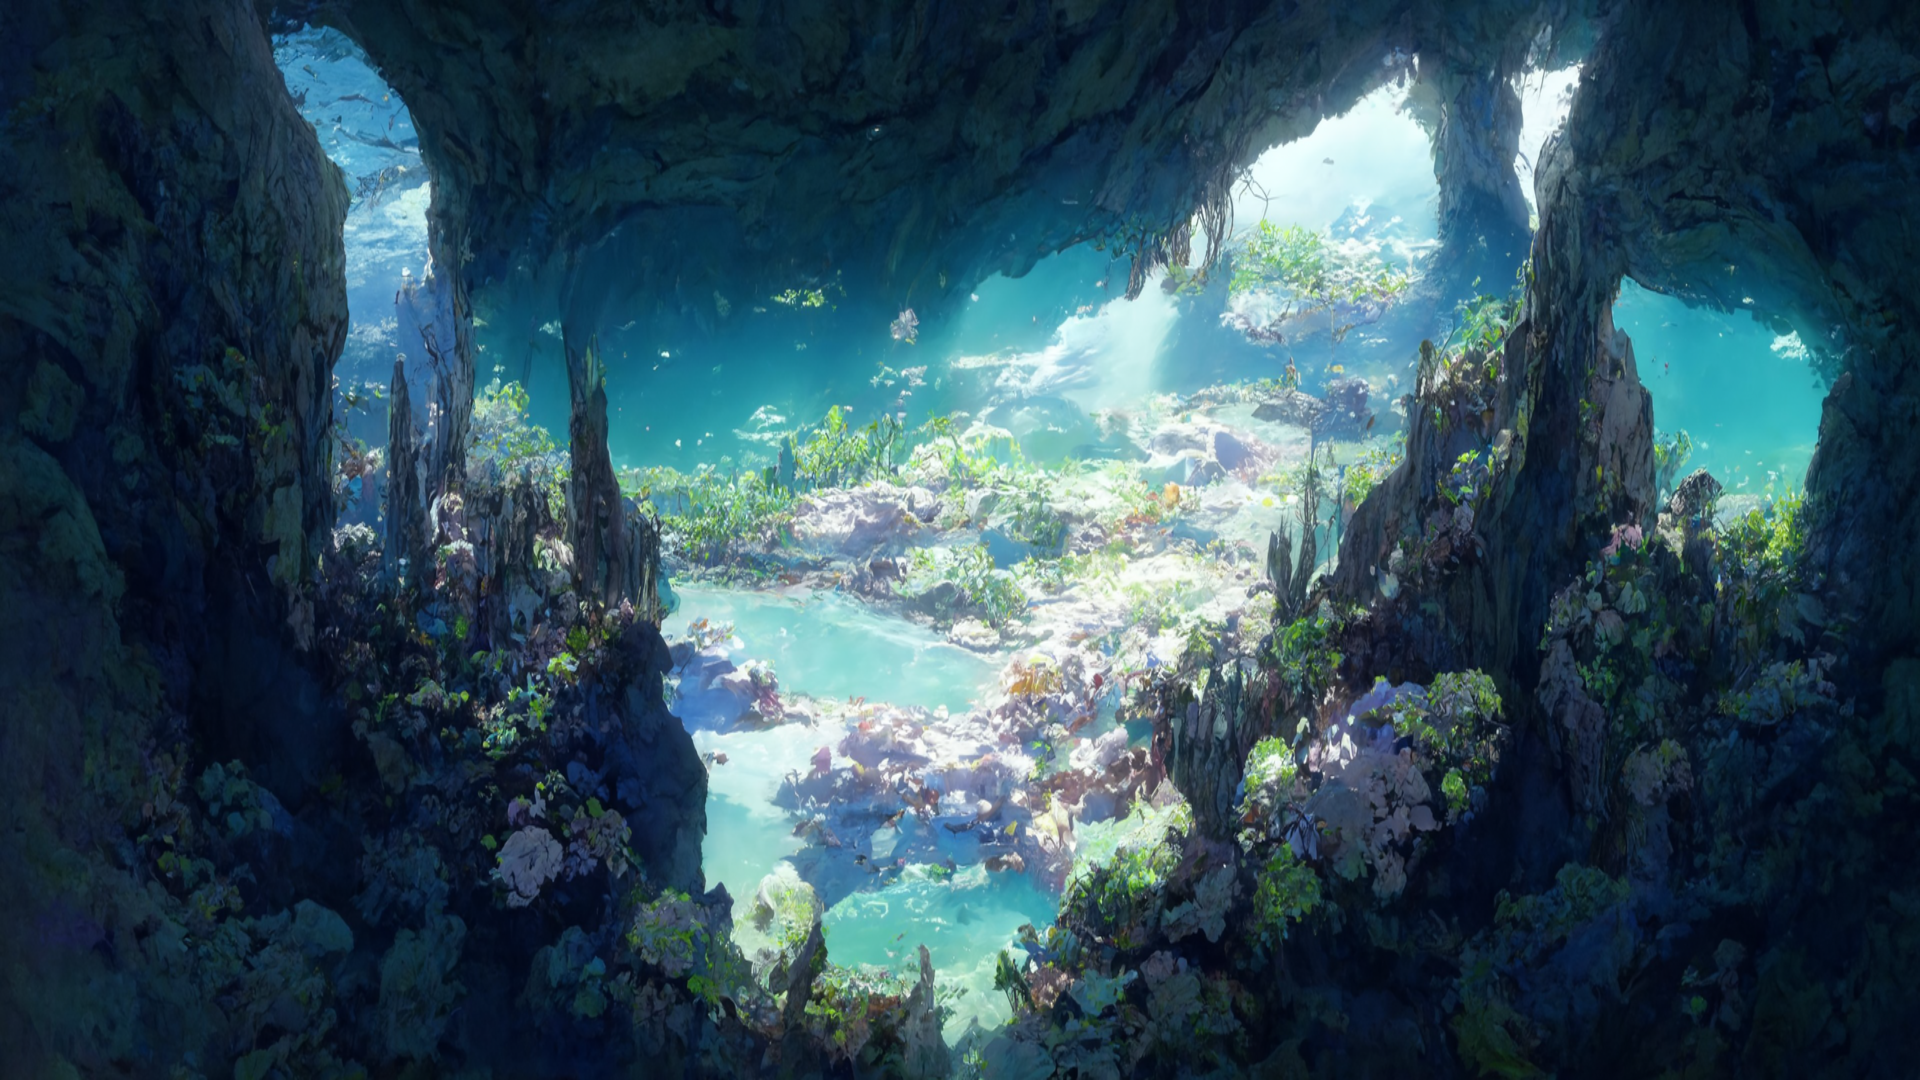
\includegraphics[width=1\textwidth]{images/background/Pixiv-100810147_p2.png}
    \end{subfigure}
    \hfill
    \begin{subfigure}{0.241\textwidth}
        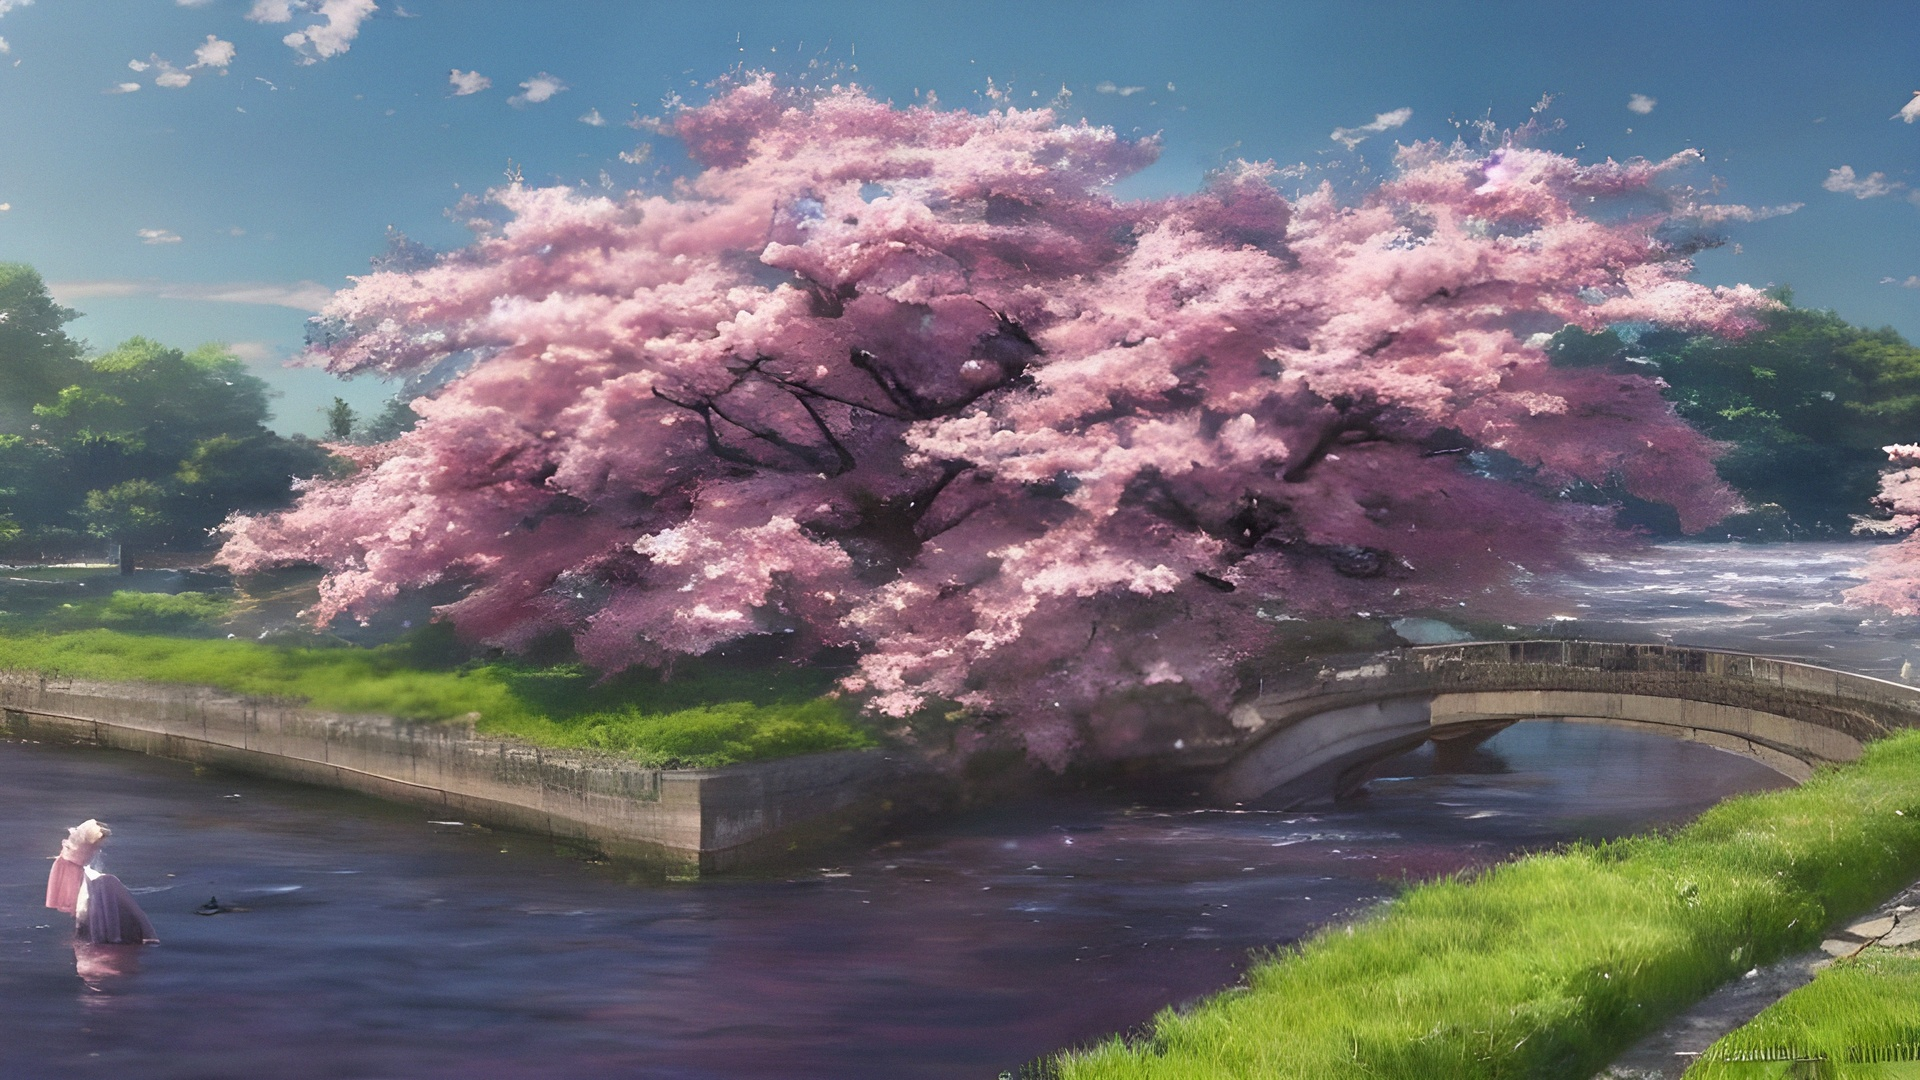
\includegraphics[width=1\textwidth]{images/background/Pixiv-101735564_p0.jpg}
    \end{subfigure}
    \hfill
    \begin{subfigure}{0.241\textwidth}
        
\includegraphics[width=1\textwidth]{images/background/Pixiv-101752160_p1.png}
    \end{subfigure}
    \caption{Background images\cite{101510980}\cite{100810147}\cite{101735564}\cite{101752160}}
\end{figure}